%
% File naaclhlt2010.tex
%
% Contact: nasmith@cs.cmu.edu

\documentclass[11pt,letterpaper]{article}
\usepackage{naaclhlt2010}
\usepackage{amsmath}
\usepackage{times}
\usepackage{latexsym}
\usepackage{graphicx}
\setlength\titlebox{6.5cm}    % Expanding the titlebox
\title{ A Machine Learning Based Approach for Predicting Adult Personal Information}

\author{Lezhong Huang\\
  Johns Hopkins University\\
  500 W. University Pkwy, 14F\\
  Baltimore, MD 21210, USA\\
  {\tt huanglezhong@gmail.com}
  \And
  Yang Dai \\
  Johns Hopkins University \\
  104 W. University Pkwy, 5F\\
  Baltimore, MD 21210, USA\\
  {\tt ydai9@jhu.edu}}

\date{}

\begin{document}
\maketitle
\begin{abstract}
This document contains how to implement a machine learning algorithm. This algorithm is applied on predicting some aspects of personal information given a large training set. The sample is a combination of many aspects of personal information, so any one of them can be selected as input. For algorithm, we divided the implementation into three stages. First is output is binary with shallow learning, and the second is multiclass output with shallow learning, and the last one is deep learning. The experiments is provided to compare the performance of the three stages.
\end{abstract}

\section{Introduction}
Intuitively, The information of one person is usually related to other information in a close range. One piece of information of a person may closely correlated with his/her other information. Besides, one person's information may also closely correlated to the information of his/her friends. Based on this trait, it's plausible to use machine learning techniques to infer one's unknown information based on other related information. In fact, 
In this paper, we have dataset of a bunch of adults' information including marital status, education, salary level and etc. We implement a machine learning system which can infer one feature of a instance based on it's other features.
\\
Generally, there are three types of machine learning tasks, supervised learning, unsupervised learning and reinforcement learning. Since the training data we have include input and output, the task in this paper is supervised learning. Based on the type of output, machine learning task can also be classified as classification, regression and clustering. In this paper, the output is either binomial or multinomial, so it is a classification task. A Neural Networks based algorithm can easily satisfy above condition. Besides, Neural networks are universal approximators, and they work well for capturing associations within a set of features, which is what we need in this task. Hence, we choose Multilayer Perceptron (MLP), which is one of feedforward artificial neural network, to implement this task.
\\
The original Multilayer Perceptron algorithm requires feature data to be discrete. However, sometimes some feature might be continuous in dataset, like the dataset we chose. In this case, we have to use an approach to transfer continuous data into discrete.
\\
The rest of this paper is organized as follows. In section 2, we briefly describe the machine learning algorithm we choose. Section 3 presents the implementation details, which introducing dataset and 3 different levels of system we implement. In section 4 we provide experiment results and system performance under different conditions. At last, we conclude the paper in section 5.

\section{Method}
The algorithm implemented in this paper is Multilayer Perceptron (MLP). MLP is an artificial nerual network to solve classificaiton problem. The bottom layer of the nerual network is input layer which consists of several input nodes, and the number of input nodes equals the number of features. The top layer of the nerual network is output layer. If the output only has two classifications, we can use only one output node, and it has binary value to represent two classifications. If the output has $N$, where $N>2$, classifications, we need $N$ nodes in output layer to represent the $N$ classifications. The layers between input layer and output layer are hidden layers. The number of hidden layers and the nodes of each hidden layers are defined by users. 
\begin{figure}[H]
\centering
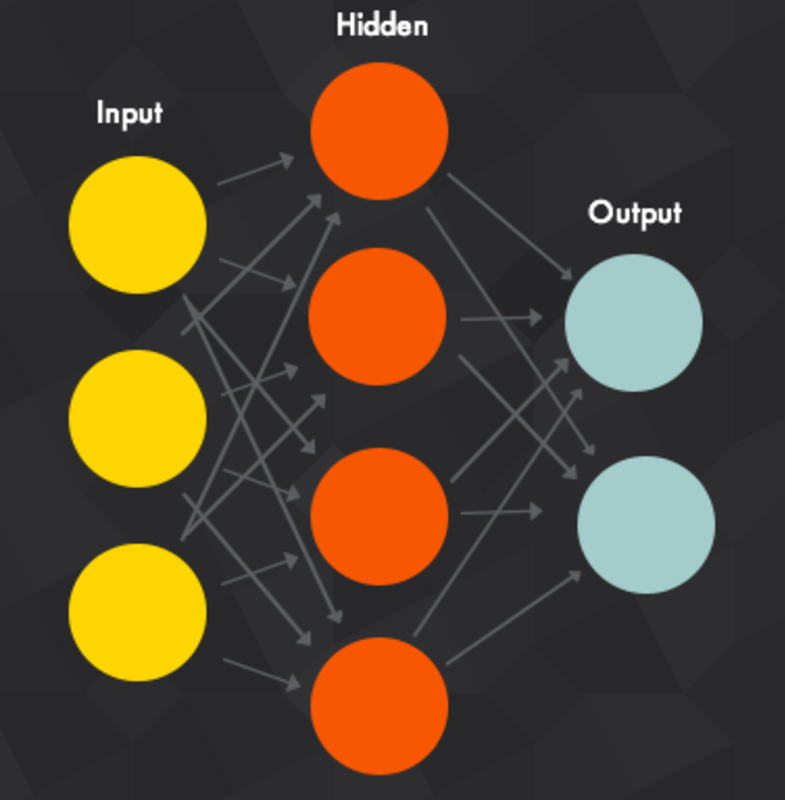
\includegraphics[scale=0.6]{deep.pdf}
\caption{\small Structure of MLP with one hidden layer}
\label{fig:structureOfMLP}
\end{figure}
The Fig.~\ref{fig:structureOfMLP} represents the structure of MLP, as shown in the figure, you can see the input layer, hidden layer and output layer. It only shows one hidden layer, although you can add more than one hidden layer according to requirements. 

\subsection{Weighted Connection}
Assume we have $M$ layers totally, including input layer and output layer. Then, the net value of each node in layer $m+1$ equals to the weighted summation of layer $m$. 
\begin{equation}
\label{eqn:netvalue}
net_j = \sum_{i \in l_m}w_{ij}net_i
\end{equation}
where $l_m$ stands for the nodes in layer $m$. As you can see in the Fig.~\ref{fig:structureOfMLP}, there are some arrows between two subsquent layers, which stand for the weighted connections. There is no connections between two nodes in the same layers. The net values of input layer is input feature, because they do not have previous layer.

\subsection{Activation Function}
For each node except the node in input layer, after getting the net value, an activation function is applied on the net value, and the result of the activation is the output of this node, which is used as the input of nodes in next layer. The activation function is an non-linear function, and in most cases, sigmoid function or hiperbolic tangent function is selected as activiation function. 
\begin{equation}
\label{eqn:sigmoid}
o_j = g(net_j) = \frac{1}{1+e^{-net_j}}
\end{equation}

\begin{equation}
\label{eqn:tanh}
o_j = g(net_j) = tanh(net_j)
\end{equation}

\subsection{Forward Propagation}
Now, we have weighted connections between two layers and activation function on each node, so we can infer the next layer given the current layer. We have input features as the input layer, then we can do forward propagation layer by layer, and finally, we get the net value of nodes in output layer. \\
We use sigmoid funciton as activation function. For binary output, we only have one output node, and we have 
\begin{equation}
\label{eqn:YEquals0}
\text{if ~~} o_j = \frac{1}{1+e^{-net_j}} < 0.5 ~~\text{then~~} Y=0
\end{equation}

\begin{equation}
\label{eqn:YEquals1}
\text{if ~~} o_j = \frac{1}{1+e^{-net_j}} \geq 0.5 ~~\text{then~~} Y=1
\end{equation}
For multiclass case which has $M$ classifications, we encode the output with $M$ nodes, and each node is still binary. For example, we have 4 classifications, we use four output nodes in output layer, and for class 1, we the values of the 4 nodes are 1000, and for class 2, 4 nodes are 0100, and for class 3, 4 nodes are 0010, and for class 4, 4 nodes are 0001. We use the same method as that of binary class case to determine the binary value of each node in output layer when training the set. 
The predict methods in training step and testing accuracy is a little bit different for multiclass case. In the training stage, it might happen that more than one node are 1, because we use 0.5 as threshold for each sigmoid function, but we only have one node equals to one in real output, so when testing the accuracy, we only let the node which has the highest value equals to one. 

\subsection{Backward Propagation}
The aim of training samples is to get appropriate weighted connections to predict accurate output. First, we use random weighted connections as initialization. Each step, an instance features are inputed and use current weighted connections to get a predicted output, and use loss function
\begin{equation}
\label{eqn:loss}
E=\frac{1}{2}(y-o_j)^2
\end{equation} 
to measure the difference between predicted result and real output, where $o_j$ means the output value of $j^{th}$ node in output layer, and $y$ is the real output. The partial derivatives of loss function on $w_{ij}$ is 
\begin{equation}
\label{eqn:partialLoss}
\frac{\partial E}{\partial w_{ij}} = \frac{\partial E}{\partial o_j} \frac{\partial o_j}{\partial net_j} \frac{\partial net_j}{\partial w_{ij}}
\end{equation}


According to equation \ref{eqn:sigmoid}, we have
\begin{equation}
\label{eqn:partialOjNetj}
\frac{\partial o_j}{\partial net_j} = g(net_j)(1-g(net_j))
\end{equation}

According to equation \ref{eqn:netvalue}, we have
\begin{equation}
\label{eqn:partialNetjNeti}
\frac{\partial net_j}{w_{ij}} = net_i
\end{equation}

If node $j$ is in output layer, according to equation \ref{eqn:loss}, we have
\begin{equation}
\label{eqn:partialEOj}
\frac{\partial E}{\partial o_j}  = o_j-y_j
\end{equation}
Thus, we have 
$$\frac{\partial E}{\partial w_{ij}} = (o_j-y_j)g(net_j)(1-g(net_j))net_i$$
let $ \frac{\partial E}{\partial o_j} \frac{\partial o_j}{\partial net_j} = \sigma_j$, we have
\begin{equation}
\label{eqn:pe}
\frac{\partial E}{\partial w_{ij}} =\sigma_jnet_i
\end{equation}

If node $j$ is not output layer, it is a little bit complicated.
\begin{equation}
\label{eqn:partialEOj2}
\frac{\partial E}{\partial o_j}  = \sum_{k \in K}(\frac{\partial E}{\partial net_k})(\frac{\partial net_k}{\partial o_j})= \sum_{k \in K}(\frac{\partial E}{\partial o_k})(\frac{\partial o_k}{\partial net_k})w_{jk}
\end{equation}
Thus, we have 
\begin{equation}
\label{eqn:pe2}
\frac{\partial E}{\partial w_{ij}} =\sigma_jnet_i
\end{equation}
where $\sigma_j = \sum_{k \in K}(\sigma_kw_{jk})g(net_j)(1-g(net_j))$
\begin{equation}
\label{eqn:deltawij}
\Delta w_{ij} = \eta \frac{\partial E}{\partial w_{ij}}
\end{equation}
where $\frac{\partial E}{\partial w_{ij}}$ is shown in equation \ref{eqn:pe} and \ref{eqn:pe2}, and $\eta$ is learning rate.

 \subsection{Pre-training}
\label{subsec:pretraining}
Pre-training is used only when there are more than one hidden layers in the network. We tried two pre-training method, one is RBM, and another is contrasive divergence(CD-1). Both of them can be applied to binary input. \\
For RBM, it is introduced and implemented in homework4, so we just use the homework4 codes. We will not talk about it here. For CD-1, the weighted connections are undirected, which means you can use the weighted connections to get lower layer nodes value according to upper layer nodes. In general, CD-1 has three steps,
\begin{enumerate}
\item use nodes $\mathbf{v}_n$ in lower layer $n$ to get nodes $\mathbf{v}_{n+1}$ in next layer $n+1$ through current weighted matrix which consists of weighted connections.
\item use the nodes $\mathbf{v}_{n+1}$ in next layer $n+1$ to get nodes $\mathbf{v}^{\prime}_n$ in lower layer $n$ through current weighted matrix.
\item use the nodes  $\mathbf{v}^{\prime}_n$ in lower layer $n$ to get nodes $\mathbf{v}^{\prime}_{n+1}$ in next layer $n+1$ through current weighted matrix.
\end{enumerate}
Now we have $\mathbf{v}_n$, $\mathbf{v}_{n+1}$, $\mathbf{v}^{\prime}_n$ and $\mathbf{v}^{\prime}_{n+1}$, and we will use them to compute new $\mathbf{w}$, where $\mathbf{w}$ is weighted matrix.
\begin{equation}
\label{cd1}
\mathbf{w_{t+1}} = \mathbf{w_t}+a(\mathbf{v_n}\mathbf{v^T_{n+1}}-\mathbf{v^{\prime}_n}\mathbf{v^{\prime T}_{n+1}})
\end{equation}
where $a$ is learning rate.\\
The initialization of $\mathbf{w}$ is randomized, and the pre-training result will be used as the initialization of training process.

\section{Implementation}
\subsection{Dataset}
We get the data set from UCI Machine Learning Repository. It contains many aspects of personal information. There are 32561 samples in training set and 16281 instances in testing set with unknown values, and if the unknown values are removed, training set has 30162 instances, and test set has 15060 instances. For binary case, we choose salary as output. If the $salary<50K$, $Y=0$, and if $salary \geq 50K$, then $Y=1$, following table shows the details about the personal features

\begin{table}[!htbp]
\caption{\small Data type of each feature, and the types after pre-processing.}

\tabcolsep = 3pt
\begin{center}
\label{tab:dataset}
\begin{small}
\begin{tabular}[c]{|c|c|c|}
%\cline{2-11}
\hline
Feature Name & Data Type & Converted Type \\
\hline
%
Age & continuous & continuous\\
\hline
Workclass & Category & Integer\\
%
\hline
Fnlwgt & continuous & continuous \\
\hline
Education & category & Integer \\
\hline
Education-num & continuous & continuous \\
\hline
Marital-status & category & Integer \\
\hline
Occupation & category & Integer \\
\hline
Relationship & category & Integer \\
\hline
Race & category & Integer \\
\hline
Sex & category & Integer \\
\hline
Capital-gain & continuous & continuous \\
\hline
Capital-loss & continuous & continuous \\
\hline
Hours-per-week & continuous & continuous \\
\hline
Native-country & category & Integer \\

\hline
\end{tabular}
\end{small}
\end{center}
\end{table}

For the multiclass case, the relationship is predicted according to other features and salary. For the category features, we assign different integer to each class from 1 to the total number of classification of that feature. After converting all the instance features to numerical, because the ranges are so different, we need to standardize these features
\begin{equation}
\label{eqn:std}
x_{ij} \gets \frac{x_{ij}-\mu_i}{s_i}
\end{equation}
where $x_{ij}$ stands for the $j^{th}$ feature of $i^{th}$ instance, and $\mu_i$ stands for the mean of $i^{th}$ feature and $s_i$ means the standard deviation of $i^{th}$ feature. All the standardization work can be done with $scale$ function in R language.

\subsection{Binary Output}
We implement the MLP algorithm by Python. Training instances are stored in a text file, and the name of the file is an input parameter. We have only one hidden layer, so the user needs to input the number of the nodes in the hidden layer. We only have one node in the output layer, which is fixed, because it is a binary output. \\
First, we need read training instances into a list, which will be used in for loop. The weighted matrices between two layers are stored in a 3-dimension list, which is initialized as an random number between 0 and 1. For each instance, we will initialize the net value of each node to zero at first, and then get a new net value after forward propagation, and all the net values are also stored in a 3-dimension list, and the list will be reset to zero when a new instance comes. In the backward propagation process, we need to store all the $\sigma_i$ in the upper layer according to equation \ref{eqn:pe2}.\\
All the weighted matrices are updeated when inputting an new instance, and after training all the instances, we can get two weighted matrices consists of weighted conncections between input layer and hidden layer and those between hidden layer and output layer. The two weighted matrices are exported to a text file, which will be used to test the accuracy of training set and testing set. \\
For testing part, we need to input file which stores the weighted matrices given by the training process, then we use forward propagation to get predicted output, and compares with real output to get the accuracy. 

\subsection{Multiclass}
Most part of multiclass is the same as binary output except the number of nodes in output layer and the difference between forward propagation and predicting process. The number of nodes in output layer equals to the number classifications, which needs to be provided by users. The forward propagation is the same as that in binary output case, but the predict process is implemented by another function to avoid more than one node in output layer equals to 1, which is impossible for real output. Thus only the node with highest value after sigmoid function equals to 1.

\subsection{Deep Learning}
The number of nodes in each hidden layer and output layer needs to be provided by users. We implement deep learning in three approaches. The first approach does not use pre-training and another two approaches use different pre-training method, one is RBM and another is CD-1. \\
For the first one which does not use pre-training, we only need to add more weighted matrices into the list which is used to store weight matrices, and other parts of the implementation is the same as multiclass.\\
For the two approaches which need pre-training, we use the first 500 samples in the training set as pre-training set, and the rest of samples are still used as training set. Also, we need do some pre-process work on the input data, because RBM and CD-1 can be only applied on binary input. First, we use sigmoid function shown in equation \ref{eqn:sigmoid} to make all the input features in the range $[0, 1]$, and use the converted value as probability in a Bernoulli trial to sample a value from $\{0, 1\}$, following is the Python code to do the pre-process work 
$$bernoulli.rvs(1.0/(1 + math.exp(-1 * x)), size=1)[0]$$
where $x$ is the data before processing. \\
For implementation of RBM, we will not talk about it here, because it has been introduced in homework4. What we did is to export the result of RBM into a file, which can be used as the initialization of the weighted matrices. \\
For the implementation of CD-1, we use the 500 samples to pre-train the weighted matrix between inputy layer and the first hidden layer, then after getting the pre-trained weighted matrix, we use it to update the value of nodes in first hidden layer. We use the same method layer by layer until we get all the pre-trained weighted matrices between two neighboring layers. As for how to get one pre-trained weighted matrix, the three steps mentioned in \ref{subsec:pretraining} are implemented. All of the vectors $\mathbf{v}_n$, $\mathbf{v}_{n+1}$, $\mathbf{v}^{\prime}_n$ and $\mathbf{v}^{\prime}_{n+1}$ are binary, and the method to convert net value to binary is the same as the pre-process method, using sigmoid function and Bernoulli trial. 

\section{Experimental Results}
The first system we implement can only infer binomial feature. The feature we choose as label is salary level, which only have two states, larger than 50k or otherwise. 

The improved system can infer feature with multinomial states. The feature we choose 


As for the final system, we use some data to do the pretraining first.


\subsection{Electronically-available resources}

NAACL HLT provides this description in \LaTeX2e{} ({\tt naaclhlt2010.tex}) and PDF
format ({\tt naaclhlt2010.pdf}), along with the \LaTeX2e{} style file used to
format it ({\tt naaclhlt2010.sty}) and an ACL bibliography style ({\tt naaclhlt2010.bst}).
These files are all available at
{\tt http://naaclhlt2010.isi.edu}.  A Microsoft Word
template file ({\tt naaclhlt2010.dot}) is also available at the same URL. We
strongly recommend the use of these style files, which have been
appropriately tailored for the NAACL HLT 2010 proceedings.


\subsection{Format of Electronic Manuscript}
\label{sect:pdf}

For the production of the electronic manuscript you must use Adobe's
Portable Document Format (PDF). This format can be generated from
postscript files: on Unix systems, you can use {\tt ps2pdf} for this
purpose; under Microsoft Windows, you can use Adobe's Distiller, or
if you have cygwin installed, you can use {\tt dvipdf} or
{\tt ps2pdf}.  Note 
that some word processing programs generate PDF which may not include
all the necessary fonts (esp. tree diagrams, symbols). When you print
or create the PDF file, there is usually an option in your printer
setup to include none, all or just non-standard fonts.  Please make
sure that you select the option of including ALL the fonts.  {\em
  Before sending it, test your {\/\em PDF} by printing it from a
  computer different from the one where it was created}. Moreover,
some word processor may generate very large postscript/PDF files,
where each page is rendered as an image. Such images may reproduce
poorly.  In this case, try alternative ways to obtain the postscript
and/or PDF.  One way on some systems is to install a driver for a
postscript printer, send your document to the printer specifying
``Output to a file'', then convert the file to PDF.

For reasons of uniformity, Adobe's {\bf Times Roman} font should be
used. In \LaTeX2e{} this is accomplished by putting

\begin{quote}
\begin{verbatim}
\usepackage{times}
\usepackage{latexsym}
\end{verbatim}
\end{quote}
in the preamble.

Additionally, it is of utmost importance to specify the {\bf
  US-Letter format} (8.5in $\times$ 11in) when formatting the paper.
When working with {\tt dvips}, for instance, one should specify {\tt
  -t letter}.

Print-outs of the PDF file on US-Letter paper should be identical to the
hardcopy version.  If you cannot meet the above requirements about the
production of your electronic submission, please contact the
publication chairs above  as soon as possible.


\subsection{Layout}
\label{ssec:layout}

Format manuscripts two columns to a page, in the manner these
instructions are formatted. The exact dimensions for a page on US-letter
paper are:

\begin{itemize}
\item Left and right margins: 1in
\item Top margin:1in
\item Bottom margin: 1in
\item Column width: 3.15in
\item Column height: 9in
\item Gap between columns: 0.2in
\end{itemize}

\noindent Papers should not be submitted on any other paper size. Exceptionally,
authors for whom it is \emph{impossible} to format on US-Letter paper,
may format for \emph{A4} paper. In this case, they should keep the \emph{top}
and \emph{left} margins as given above, use the same column width,
height and gap, and modify the bottom and right margins as necessary.
Note that the text will no longer be centered.

\subsection{The First Page}
\label{ssec:first}

Center the title, author's name(s) and affiliation(s) across both
columns. Do not use footnotes for affiliations.  Do not include the
paper ID number assigned during the submission process. 
Use the two-column format only when you begin the abstract.

{\bf Title}: Place the title centered at the top of the first page, in
a 15 point bold font.  (For a complete guide to font sizes and styles, see Table~\ref{font-table}.)
Long title should be typed on two lines without
a blank line intervening. Approximately, put the title at 1in from the
top of the page, followed by a blank line, then the author's names(s),
and the affiliation on the following line.  Do not use only initials
for given names (middle initials are allowed). Do not format surnames
in all capitals (e.g., ``Leacock,'' not ``LEACOCK'').  The affiliation should
contain the author's complete address, and if possible an electronic
mail address. Leave about 0.75in between the affiliation and the body
of the first page.

{\bf Abstract}: Type the abstract at the beginning of the first
column.  The width of the abstract text should be smaller than the
width of the columns for the text in the body of the paper by about
0.25in on each side.  Center the word {\bf Abstract} in a 12 point
bold font above the body of the abstract. The abstract should be a
concise summary of the general thesis and conclusions of the paper.
It should be no longer than 200 words.  The abstract text should be in 10 point font.

{\bf Text}: Begin typing the main body of the text immediately after
the abstract, observing the two-column format as shown in 
the present document.  Do not include page numbers.

{\bf Indent} when starting a new paragraph. For reasons of uniformity,
use Adobe's {\bf Times Roman} fonts, with 11 points for text and 
subsection headings, 12 points for section headings and 15 points for
the title.  If Times Roman is unavailable, use {\bf Computer Modern
  Roman} (\LaTeX2e{}'s default; see section \ref{sect:pdf} above).
Note that the latter is about 10\% less dense than Adobe's Times Roman
font.

\subsection{Sections}

{\bf Headings}: Type and label section and subsection headings in the
style shown on the present document.  Use numbered sections (Arabic
numerals) in order to facilitate cross references. Number subsections
with the section number and the subsection number separated by a dot,
in Arabic numerals. 

{\bf Citations}: Citations within the text appear
in parentheses as~\cite{Gusfield:97} or, if the author's name appears in
the text itself, as Gusfield~\shortcite{Gusfield:97}. 
Append lowercase letters to the year in cases of ambiguities.  
Treat double authors as in~\cite{Aho:72}, but write as 
in~\cite{Chandra:81} when more than two authors are involved. 
Collapse multiple citations as in~\cite{Gusfield:97,Aho:72}.

\textbf{References}: Gather the full set of references together under
the heading {\bf References}; place the section before any Appendices,
unless they contain references. Arrange the references alphabetically
by first author, rather than by order of occurrence in the text.
Provide as complete a citation as possible, using a consistent format,
such as the one for {\em Computational Linguistics\/} or the one in the 
{\em Publication Manual of the American 
Psychological Association\/}~\cite{APA:83}.  Use of full names for
authors rather than initials is preferred.  A list of abbreviations
for common computer science journals can be found in the ACM 
{\em Computing Reviews\/}~\cite{ACM:83}.

The \LaTeX{} and Bib\TeX{} style files provided roughly fit the
American Psychological Association format, allowing regular citations, 
short citations and multiple citations as described above.

{\bf Appendices}: Appendices, if any, directly follow the text and the
references (but see above).  Letter them in sequence and provide an
informative title: {\bf Appendix A. Title of Appendix}.

\textbf{Acknowledgment} sections should go as a last (unnumbered) section immediately
before the references.  

\subsection{Footnotes}

{\bf Footnotes}: Put footnotes at the bottom of the page. They may
be numbered or referred to by asterisks or other
symbols.\footnote{This is how a footnote should appear.} Footnotes
should be separated from the text by a line.\footnote{Note the
line separating the footnotes from the text.}  Footnotes should be in 9 point font.

\subsection{Graphics}

{\bf Illustrations}: Place figures, tables, and photographs in the
paper near where they are first discussed, rather than at the end, if
possible.  Wide illustrations may run across both columns and should be placed at
the top of a page. Color illustrations are discouraged, unless you have verified that 
they will be understandable when printed in black ink.

\begin{table}
\begin{center}
\begin{tabular}{|l|rl|}
\hline \bf Type of Text & \bf Font Size & \bf Style \\ \hline
paper title & 15 pt & bold \\
author names & 12 pt & bold \\
author affiliation & 12 pt & \\
the word ``Abstract'' & 12 pt & bold \\
section titles & 12 pt & bold \\
document text & 11 pt  &\\
abstract text & 10 pt & \\
captions & 10 pt & \\
bibliography & 10 pt & \\
footnotes & 9 pt & \\
\hline
\end{tabular}
\end{center}
\caption{\label{font-table} Font guide. }
\end{table}

{\bf Captions}: Provide a caption for every illustration; number each one
sequentially in the form:  ``Figure 1. Caption of the Figure.'' ``Table 1.
Caption of the Table.''  Type the captions of the figures and 
tables below the body, using 10 point text.  

\section{Length of Submission}
\label{sec:length}

The NAACL HLT 2010 main conference accepts submissions of long papers
and short papers.  The maximum length of a long paper manuscript is
eight (8) pages of content and one (1) additional page of references
\emph{only} (appendices count against the eight pages, not the
additional one page).  The maximum length of a short paper manuscript
is four (4) pages including references.  For both long and short
papers, all illustrations, references, and appendices must be
accommodated within these page limits, observing the formatting
instructions given in the present document.  Papers that do not
conform to the specified length and formatting requirements are
subject to be rejected without review.

% Up to two (2) additional pages may be purchased from ACL at the
% price of \$250 per page; please contact the publication chairs above
% for more information about this option.

\section*{Acknowledgments}

Do not number the acknowledgment section.

\begin{thebibliography}{}


\bibitem[\protect\citename{Aho and Ullman}1972]{Aho:72}
Alfred~V. Aho and Jeffrey~D. Ullman.
\newblock 1972.
\newblock {\em The Theory of Parsing, Translation and Compiling}, volume~1.
\newblock Prentice-{Hall}, Englewood Cliffs, NJ.

\bibitem[\protect\citename{{American Psychological Association}}1983]{APA:83}
{American Psychological Association}.
\newblock 1983.
\newblock {\em Publications Manual}.
\newblock American Psychological Association, Washington, DC.

\bibitem[\protect\citename{{Association for Computing Machinery}}1983]{ACM:83}
{Association for Computing Machinery}.
\newblock 1983.
\newblock {\em Computing Reviews}, 24(11):503--512.

\bibitem[\protect\citename{Chandra \bgroup et al.\egroup }1981]{Chandra:81}
Ashok~K. Chandra, Dexter~C. Kozen, and Larry~J. Stockmeyer.
\newblock 1981.
\newblock Alternation.
\newblock {\em Journal of the Association for Computing Machinery},
  28(1):114--133.

\bibitem[\protect\citename{Gusfield}1997]{Gusfield:97}
Dan Gusfield.
\newblock 1997.
\newblock {\em Algorithms on Strings, Trees and Sequences}.
\newblock Cambridge University Press, Cambridge, UK.

\end{thebibliography}

\end{document}
